\documentclass[12pt]{article}
\usepackage[utf8]{inputenc}
\usepackage[a4paper,margin=1in]{geometry}
\usepackage{amsmath} 
\usepackage{amssymb}
\usepackage{graphicx}
\usepackage{float}
\usepackage{tabularx} 
\usepackage{caption}
\usepackage{subcaption}
\usepackage{array}
\usepackage{listings}
\usepackage{pythonhighlight}



\title{
    Department Of Aerospace Engineering,\\
    Indian Institute Of Technology Madras
    \begin{figure}[H]
        \centering
        
\includegraphics[width=8cm]{iitmlogo.png}
    \end{figure}
    \begin{center}
        \textbf{\\AS2101 : Introduction to Aerospace Engineering\\}
        Report 7 : QR Decomposition\\
    \end{center}
}
\author{
    Pranit Zope\\AE20B046
}
\date{\today}

\begin{document}
\pagenumbering{gobble}
\maketitle
\newpage
\pagenumbering{arabic}
\tableofcontents 
\listoffigures

\newpage
\section{Aim}
To decompose a square matrix A of order n into an orthogonal matrix Q and upper triangle matrix R and solve linear equations.

\section{Theory}
QR Decomposition is a method of decomposing a matrix A into two matrices Q and R,  Q being an orthogonal matrix and R being an upper triangular matrix. We eill use \textbf{Eigenvalue Algorithm} to solve this problem.\\
This method only works for invertible matrices and is very useful in solveing linear equations of the form AX=B.3

\subsection{Procedure for finding Q and R}
Let us consider a matrix A given to us.
\begin{equation*}
    \mathbf{A}=\left[\mathbf{a}_{1} \mathbf{a}_{2} \mathbf{a}_{3} \mathbf{a}_{4} \ldots \mathbf{a}_{\mathbf{n}}\right]
\end{equation*}
Now, we need to find Q which is orthogonal. So, we will use the Grahm-Schmidt Algorithm to find Q.\\
Thus, 
\begin{equation*}
    \mathrm{q}_{1}=\frac{\mathrm{a}_{1}}{\left\|\mathrm{a}_{1}\right\|}
\end{equation*}
To find q2 we need to take a2 and remove the component along q1 to make it perpendicular to q1, i.e orthogonal and then normalise.
\begin{equation*}
    \mathrm{q}_{2}=\frac{\mathrm{a}_{2}-<\mathrm{a}_{2}, \mathrm{q}_{1}>\mathrm{q}_{1}}{\left\|\mathrm{a}_{2}-<\mathrm{a}_{2}, \mathrm{q}_{1}>\mathrm{q}_{1}\right\|}
\end{equation*}
Similarly, for q3; 
\begin{equation*}
    \mathrm{q}_{3}=\frac{\mathrm{a}_{3}-<\mathrm{a}_{3}, \mathrm{q}_{2}>\mathrm{q}_{2}-<\mathrm{a}_{3}, \mathrm{q}_{1}>\mathrm{q}_{1}}{\left\|\mathrm{a}_{3}-<\mathrm{a}_{3}, \mathrm{q}_{2}>\mathrm{q}_{2}-<\mathrm{a}_{3}, \mathrm{q}_{1}>\mathrm{q}_{1}\right\|}
\end{equation*}
and doing the same for $q_n$ ;
\begin{equation*}
    \mathrm{q}_{\mathrm{n}}=\frac{\mathrm{a}_{\mathrm{n}}-\sum_{\mathrm{i}=1}^{\mathrm{n}-1}<\mathrm{a}_{3}, \mathrm{q}_{\mathrm{i}}>\mathrm{q}_{\mathrm{i}}}{\left\|\mathrm{a}_{\mathrm{n}}-\sum_{\mathrm{i}=1}^{\mathrm{n}-1}<\mathrm{a}_{3}, \mathrm{q}_{\mathrm{i}}>\mathrm{q}_{\mathrm{i}}\right\|}
\end{equation*}
\\
Now that we have $Q$
\begin{equation*}
    \mathbf{Q}=\left[\mathbf{q}_{1} \mathbf{q}_{2} \mathbf{q}_{3} \mathbf{q}_{4} \ldots \mathbf{q}_{\mathbf{n}}\right]
\end{equation*}

Now we will write $a_i$ in terms of $q_i$;
\begin{equation*}
    a_{i}=\sum_{j=1}^{j=i}<a_{i}, q_{j}>q_{j}
\end{equation*}
For factorisation, the coefficients of qi must form column vectors in the matrix R.\\
Hence we can say that R will be:
\begin{equation*}
    \left[\begin{array}{ccccc}
< a_{1}, q_{1}> & <a_{2}, q_{1}> & \ldots & \ldots & < a_{n}, q_{1}> \\
<a_{1}, q_{2}> & <a_{2}, q_{2}> & \ldots & \ldots & <a_{n}, q_{2}> \\
\ldots & \ldots & \ldots & \ldots & \ldots \\
\ldots & \ldots & \ldots & \ldots & \ldots \\
< a_{n}, q_{1}> & <a_{n}, q_{2}> & \ldots & \ldots & <a_{n}, q_{n}>
\end{array}\right]
\end{equation*}
Since there is no component of $a_i$ about $q_j$, $j>i$, R takes the form of upper triangular matrix as others take the value 0.
\begin{equation*}
    R=\left[\begin{array}{ccccc}
<a_{1}, q_{1}> & <a_{2}, q_{1}> & \ldots & \ldots & <a_{n}, q_{1}> \\
0 & <a_{2}, q_{2}> & \ldots & \ldots & <a_{n}, q_{2}> \\
\ldots & \ldots & \ldots & \ldots & \ldots \\
\ldots & \ldots & \ldots & \ldots & \ldots \\
0 & 0 & \ldots & \ldots & <a_{n}, q_{n}>
\end{array}\right]
\end{equation*}

\subsection{Solving Linear Equations using this}
Lets say we have $AX=B$ linear equaiton. Using the QR Decompostion, we have $A=QR$\\
Thus, 
\begin{equation*}
    QRX=B
\end{equation*}
\begin{equation*}
    RX=Q^{-1}B
\end{equation*}
Since Q is orthogonal, $Q^{-1} = Q^T$, Thus we have
\begin{equation*}
    RX=Q^TB
\end{equation*}
Now, since R is a upper triangular matrix, we can solve this by back substitution -
\begin{equation*}
    \left[\begin{array}{c}
\sum_{i=1}^{n} r_{1, i} x_{i} \\
. . \\
. . \\
r_{(n-1) n} x_{n}+r_{n-1, n-1} x_{n-1} \\
r_{n n} x_{n}
\end{array}\right]=\left[\begin{array}{c}
k_{1} \\
. . \\
. . \\
k_{n-1} \\
k_{n}
\end{array}\right]
\end{equation*}
From here,  we obtain $x_1,x_2,x_3,...,x_n$ without any complicated solving.
\newpage

\section{Verification of the Method}
Previously in this course, we had linearly regressed a data to obtain a best fitting line. We will use the same dataset to validate the QR- Decomposition method.

For "data2.txt", using linear regression, we got the slope as
\begin{python}
m = 2.0056244629115776
c = 1.3809824773861692
\end{python}
Now, using the QR method,  we get the following output :
\begin{python}
x1 =

   2.0056
   1.3810
\end{python}
The former line being the slope and later the intercept.\\
Thus, we can say that the result we got in both the methods is same.

\section{Efficiency comparision of several Methods}
We will now compare several method of soving the linear equations using a graph
\begin{figure}[H]
    \centering
    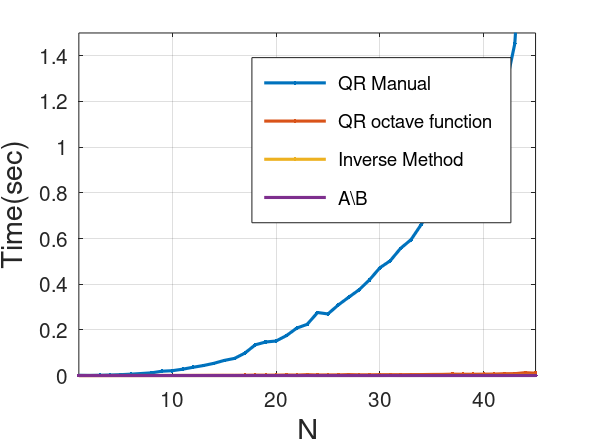
\includegraphics[width=10cm]{n_time.png}
    \caption{Comparision of time taken in different methods}
\end{figure}
\newpage
Also, we can compare the time taken at each steap and the total time :
\begin{figure}[H]
    \centering
    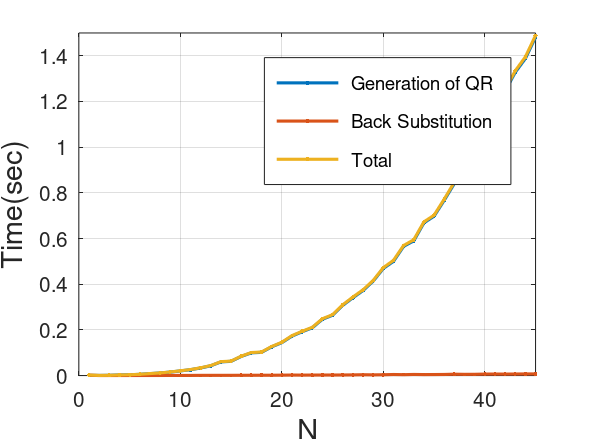
\includegraphics[width=10cm]{manual_time.png}
    \caption{Time taken at each step and the total time}
\end{figure}

\section{Result and Conclusion}
We can see that the time taken in the Generation of QR is a lot. Hence,  this method is simpler but takes a lot of time for the computer.\\
A possible reason for this is that the algorithm is very bulky as it involves calculating multiple $n\times n$ matrices.\\
Thus we can conclude that the method is correct, works fine. Also, it is not sufficient for a computer program since the time of computation is very high.

\end{document}